% Template created by Karol Kozioł (www.karol-koziol.net) for ShareLaTeX

\documentclass[a4paper,9pt]{extarticle}
\usepackage[utf8]{inputenc}
\usepackage[T1]{fontenc}
\usepackage{graphicx}
\usepackage{xcolor}
\usepackage{tikz}

\usepackage{listings}
\lstset{basicstyle=\ttfamily,
  showstringspaces=false,
  commentstyle=\color{red},
  keywordstyle=\color{blue}
}



\usepackage{amsmath,amssymb,textcomp}
\everymath{\displaystyle}

\usepackage{times}
\renewcommand\familydefault{\sfdefault}
\usepackage{tgheros}
\usepackage[defaultmono,scale=0.85]{droidmono}

\usepackage{multicol}
\setlength{\columnseprule}{0pt}
\setlength{\columnsep}{20.0pt}


\usepackage{geometry}
\geometry{
a4paper,
total={210mm,297mm},
left=10mm,right=10mm,top=10mm,bottom=15mm}

\linespread{1.3}


% custom title
\makeatletter
\renewcommand*{\maketitle}{%
\noindent
\begin{minipage}{0.4\textwidth}

\begin{tikzpicture}
\node[rectangle,rounded corners=6pt,inner sep=10pt,fill=blue!60!green,text width= 0.95\textwidth] {\color{white}\Huge \bf \@title};
\end{tikzpicture}
\end{minipage}
\hfill
\begin{minipage}{0.55\textwidth}
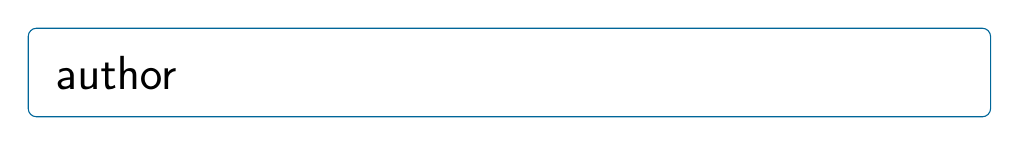
\begin{tikzpicture}
\node[rectangle,rounded corners=3pt,inner sep=10pt,draw=blue!60!green,text width= 0.95\textwidth] {\LARGE \@author};
\end{tikzpicture}
\end{minipage}
\bigskip\bigskip
}%
\makeatother

% custom section
\usepackage[explicit]{titlesec}
\newcommand*\sectionlabel{}
\titleformat{\section}
  {\gdef\sectionlabel{}
   \normalfont\sffamily\Large\bfseries\scshape}
  {\gdef\sectionlabel{\thesection\ }}{0pt}
  {
\noindent
\begin{tikzpicture}
\node[rectangle,rounded corners=3pt,inner sep=4pt,fill=blue!60!green,text width= 0.95\columnwidth] {\color{white}\sectionlabel#1};
\end{tikzpicture}
  }
\titlespacing*{\section}{0pt}{15pt}{10pt}


% custom footer
\usepackage{fancyhdr}
\makeatletter
\pagestyle{fancy}
\fancyhead{}
\fancyfoot[C]{\footnotesize \textcopyright\ \@author. \ \@date}
\renewcommand{\headrulewidth}{0pt}
\renewcommand{\footrulewidth}{0pt}
\makeatother


\title{Git CheatSheet}
\author{Fawaz Alazemi}
\date{Last update:\today}



\begin{document}

\maketitle

\begin{multicols*}{2}
\section{Setup}
Clone an existing repository
\begin{lstlisting}[language=bash]
$ git clone https://address.git
\end{lstlisting}
Create an empty local repository
\begin{lstlisting}[language=bash]
$ git init 
\end{lstlisting}
Add author name and email
\begin{lstlisting}[language=bash]
$ git config --global user.name "Fawaz M."
$ git config --global user.email Fawaz@Fawaz.com
\end{lstlisting}
Ignore files/directories
\begin{lstlisting}[language=bash]
$ vim .gitignore #add files description 
$ git add .gitignore;
$ git commit -m "ignore description"
\end{lstlisting}

%%%%%%%%%%%%%%%%%%%%%%%%%%%%%%%%%%%%%%%%%%%%

\section{Local Changes}
Check status (uncommitted file changes, addition, or deletion)
\begin{lstlisting}[language=bash]
$ git status
\end{lstlisting}
Stage all current changes
\begin{lstlisting}[language=bash]
$ git add .
\end{lstlisting}
Commit your staged files with long message  
\begin{lstlisting}[language=bash]
$ git commit
\end{lstlisting}
Commit staged files with a short message
\begin{lstlisting}[language=bash]
$ git commit -m "Message"
\end{lstlisting}
Amend the last commit message
\begin{lstlisting}[language=bash]
$ git commit --amend -m "Amendment"
\end{lstlisting}

%%%%%%%%%%%%%%%%%%%%%%%%%%%%%%%%%%%%%%%%%%%%

\section{History}
Show all commits
\begin{lstlisting}[language=bash]
$ git log
\end{lstlisting}
Show most n commits
\begin{lstlisting}[language=bash]
$ git log -n
\end{lstlisting}
Show online for each commit
\begin{lstlisting}[language=bash]
$ git log --oneline 
\end{lstlisting}

\end{multicols*}

\end{document}
